%# -*- coding: utf-8-unix -*-
%======================================================================
% qbook.tex for Qbook Template
%======================================================================
% 双面打印
\documentclass{qbook}
\addbibresource{bib/GW_DA.bib}  % 导入参考文献数据库
\begin{document}
\pagestyle{empty}
%# -*- coding: utf-8-unix -*-
\thispagestyle{empty}
\begin{tikzpicture}[overlay,remember picture,font=\sffamily\bfseries]
\draw[ultra thick,c4,name path=big arc] ([xshift=-2mm]current page.north) arc(150:285:11)
coordinate[pos=0.225] (x0);
\begin{scope}
\clip ([xshift=-2mm]current page.north) arc(150:285:11) --(current page.north
east);
\fill[c4!50,opacity=0.25] ([xshift=4.55cm]x0) circle (4.55);
\fill[c4!50,opacity=0.25] ([xshift=3.4cm]x0) circle (3.4);
\fill[c4!50,opacity=0.25] ([xshift=2.25cm]x0) circle (2.25);
\draw[ultra thick,c4!50] (x0) arc(-90:30:6.5);
\draw[ultra thick,c4] (x0) arc(90:-30:8.75);
\draw[ultra thick,c4!50,name path=arc1] (x0) arc(90:-90:4.675);
\draw[ultra thick,c4!50] (x0) arc(90:-90:2.875);
\path[name intersections={of=big arc and arc1,by=x1}];
\draw[ultra thick,c4,name path=arc2] (x1) arc(135:-20:4.75);
\draw[ultra thick,c4!50] (x1) arc(135:-20:8.75);
\path[name intersections={of=big arc and arc2,by={aux,x2}}];
\draw[ultra thick,c4!50] (x2) arc(180:50:2.25);
\end{scope} 
\path[decoration={text along path,text color=c4,
	raise = -2.8ex,
	text  along path,
	text = {|\sffamily\bfseries|\today},
	text align = center,
},
decorate
] ([xshift=-2mm]current page.north) arc(150:245:11);
%
\begin{scope}
\path[clip,postaction={fill=c3}]
([xshift=2cm,yshift=-8cm]current page.center) rectangle ++ (4.2,7.7);
\fill[c2] ([xshift=0.5cm,yshift=-8cm]current page.center)
([xshift=0.5cm,yshift=-8cm]current page.center)  arc(180:60:2)
|- ++ (-3,6) --cycle;
\draw[ultra thick,c4] ([xshift=-1.5cm,yshift=-8cm]current page.center) 
arc(180:0:2);
\draw[ultra thick,c4] ([xshift=0.5cm,yshift=-8cm]current page.center) 
arc(180:0:2);
\draw[ultra thick,c4] ([xshift=2.5cm,yshift=-8cm]current page.center) 
arc(180:0:2);
\draw[ultra thick,c4] ([xshift=4.5cm,yshift=-8cm]current page.center) 
arc(180:0:2);
\fill[red] ([xshift=2.5cm,yshift=-8cm]current page.center) +(60:2) circle(1.5mm);
  \node[text=c5!80!black] at ([xshift=4.7cm,yshift=-5.2cm]current page.center) {$G_{\mu \nu}=  \frac{8\pi G}{c^4}T_{\mu \nu}$};
\end{scope}
%
\fill[c1] ([xshift=2cm,yshift=-8cm]current page.center) rectangle ++ (-13.7,7.7);
\node[text=white,anchor=west,scale=4,inner sep=0pt] at
  ([xshift=-10.55cm,yshift=-3cm]current page.center) {引力波数据处理};
\node[text=white,anchor=west,scale=2,inner sep=0pt] at
([xshift=-4.5cm,yshift=-5.5cm]current page.center) {胡一鸣};
\end{tikzpicture}
  % 载入封面
\input{tex/tag.tex}
\newcommand{\GR}{广义相对论}
\newcommand{\SR}{狭义相对论}
\newcommand{\gw}{引力波}
\newcommand{\DA}{数据处理}

\begin{center}
        %% ----- input git-version tag
        git \commitID\\
        编译日期:\commitDATE\\
	\Large{\sffamily\bfseries\heiti 任何建议及错误信息请发送至邮箱} \\
        \texttt{\href{mailto:huyiming@sysu.edu.cn}{huyiming@sysu.edu.cn}}
\end{center} 
\vfill

\begin{figure}[htp]
\centering

\includegraphics[width=0.5\textwidth]{QR_code.png}
\label{fig:QRcode}
\end{figure}

\vspace{10em}
\begin{tabular*}{\textwidth}{ccc}
	\includegraphics{figure/by-nc.eps}
	& \begin{minipage}[b]{0.7\textwidth}
		\small\sffamily
                本作品采用知识共享 署名 4.0 国际 许可协议进行许可. 访问\url{https://creativecommons.org/licenses/by/4.0/}查看该许可协议。\\
本作品\LaTeX 模板采用\footnote{https://github.com/muzimuzhi/Qbook},遵守知识共享 署名-非商业性使用 4.0 国际 许可协议进行许可。访问\url{https://creativecommons.org/licenses/by-nc/4.0/}查看该许可协议。
	\end{minipage}
\end{tabular*}  
\thispagestyle{empty}
\frontmatter  % 对前言和概览用罗马数字作为页码
\pagestyle{empty}

\begin{pre}
	\thispagestyle{empty}
          {\kaishu{
          
          Joseph Weber是引力波探测的先驱。他建造了两个相隔上千公里的探测器,这样就可以有效地隔绝环境噪声产生的误警(实际上,LIGO也是遵从这样的宗旨选址的),因为引力波的传播速度是光速,所以两个探测器应该近乎同时探测到信号;而噪声的到来对不同的探测器则是相互独立的。Weber记录的数据中,就有几个信号,不同的探测器记录的时间差非常短。
          1969年,Weber在{\emph Physical Review Letters}上发表论文“Evidence for discovery of gravitational radiation”,宣称发现了引力波信号。一时间,他名声鹊起,成为了聚光灯前的宠儿,媒体将其捧为继Einstein之后最伟大的物理学家。

          2017年,三位物理学家由于引力波的发现而获得诺贝尔奖。三个人里,没有Weber。当然,斯人已去,Weber在世纪之交的2000年9月30日就已作古。然而,Weber与诺奖失之交臂,并不是因为他活的不够长——这一点日渐成为获得诺奖的必要非充分条件——而是因为后续的研究无法重复Weber的结论。先是理论计算结果与Weber宣称的引力波信号强度、频次相差悬殊;接着,其他团队建造的更灵敏的探测器宣布无法探测到引力波事件;最致命的是,Weber在相隔三个时区的两个信号中寻找同时信号的时候,竟然忘了考虑时差。

          Weber是真诚的,直到他去世时,他依然坚信他成功地探测到了引力波。这里并没有学术不端,有的,只是对数据处理的极度忽视。当然,也许,Weber数据处理地好一些,就不会引发这么大的轰动,也就不会吸引这么多聪明人投身到引力波探测这个领域,也许2015年9月14日穿越地球而过的那一串小小涟漪,就会如它之前的所有双黑洞并合的信号般,悄悄地来,又悄悄地去,不留下意思痕迹。

          2016年,引力波探测的大门,已然被叩开,黑洞与中子星疯狂的舞蹈终于觅来了知音。在2019年的这个夏天,当我远眺未来,充满的是憧憬和期待,当天琴卫星上天,当宇宙的长波电台被天琴接收到信号时,又会上演什么样的一出好戏呢?科学的魅力往往就在于它的不可捉摸和不可预测。不管是什么样的发现,背后一定会有着有力的数据处理方法作为支撑。还好,卫星上的时钟同步用的是原子钟,应该不至于忘记考虑时差这回事。

          历史不容假设,当我们回望过去的时候,我们也许会将Weber铭记为一位勇敢的先驱,一位卓绝的工程师,甚或是一位天才的实验物理学家;但同时,不容否认,他在引力波数据处理这门课上,表现地糟糕透了。
          我相信,当未来的人们回望这段当前,回顾中国科学的崛起时,引力波探测、天琴计划,都会是绕不过去的、在历史的长河中熠熠发光的名字。我们有着国内顶尖的激光团队,国内顶尖的惯性基准团队,国内顶尖的卫星系统团队。我希望,我们也将会有国内顶尖的引力波数据处理团队。

          这段历史画卷,现在就将由你谱写。
          愿这一本讲义,能成为你的画笔,你的颜料。

          愿原力与你同在。
          }}

%\vspace*{5\baselineskip}
%\centerline{\includegraphics[scale=0.6]{example/gzh.jpg}}
%\centerline{\fontsize{26pt}{26pt} 微信公众号}
\end{pre}

\pagestyle{empty}
\tableofcontents
\cleardoublepage
%# -*- coding: utf-8-unix -*-
\begin{overview}
\thispagestyle{empty}

这份讲义是我为中山大学物理与天文学院研究生课程“引力波数据处理”课程所准备的。
由于本人能力有限,准备时间仓促,一定包含了大量错误,我会力争在收到反馈之后进行更正。
讲义的电子版可以在\url{https://github.com/yiminghu-SYSU/GW_DA_notes}获得。

这本讲义的写作对象是对引力波数据处理感兴趣的高年级本科生或研究生。
本书默认读者已经初步掌握了狭义相对论的基本概念,并有一定概率论基础。
在讲义中,我会尽可能追求内容的完整性,以便尚未完成广义相对论等课程学习的同学也可以在脑中构建起足够的物理图景。

但限于篇幅和授课计划,本书肯定无法替代广义相对论等基础课程。
因此,文中肯定会在数学逻辑的严谨性和课程主题的完备性之间做出倾向于后者的取舍,也敬请诸位谅解。

  \rightline{\kaishu{胡一鸣}}
  \rightline{\kaishu{2019年8月14日,于珠海唐家}}
\end{overview}
 
\mainmatter	  % 对正文用阿拉伯数字作为页码
%======================================================================
% 正文内容
\pagestyle{fancy}
\setcounter{page}{0}
%# -*- coding: utf-8-unix -*-
%%==================================================
\chapter{相对论基础}

本讲义的授课主题,是\gw\DA,共分为两部分,\emph{\gw}与\emph{\DA}。
如果脱离了\gw 的物理图景,而直接空谈\DA,未免空中楼阁。
而在另一方面,引力波又是Einstein广义相对论的直接理论预言,因此,引力波的理论描述,无法跳脱广义相对论的框架。

\begin{figure}[htp]
\centering
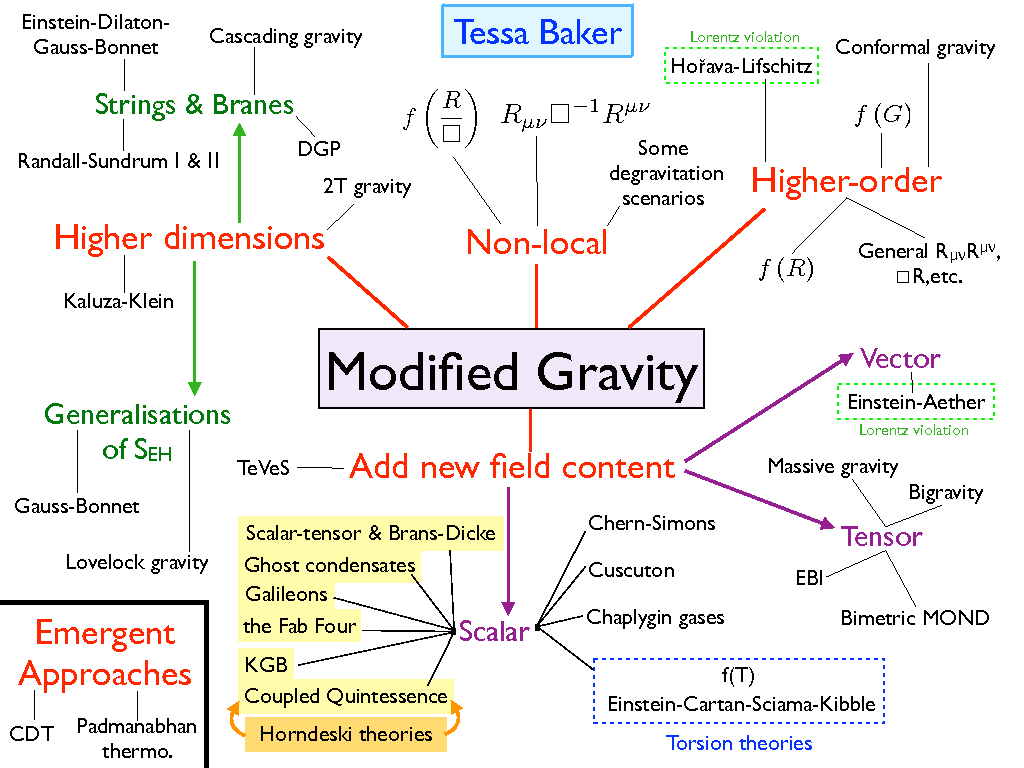
\includegraphics[width=0.7\textwidth]{ModifiedGravity.png}
\bicaption{修改引力理论}
  {Theories of modified gravity. Credit: http://www.cgc-yzu.cn/Upload/research/MG-20240317524.png}
\label{fig:ModGrav}
\end{figure}

从Einstein至今,引力理论已经有了长足的发展,如图\ref{fig:ModGrav}所示,仅基于\GR 基础上发展起来的修改引力理论就已不计其数。
由于和量子力学原理的深刻矛盾,有理由认为Einstein决定论性的的\GR 在某个地方一定背离了引力的物理本质。
然而,时至今日,Einstein昔日基于\GR 所作出的诸多预言,一一被实验所验证;所有可靠的实验检验下,\GR 均可以给出解释——而它通常是最简洁的那个理论。
因此,即使将来的实验证明了\GR 与引力的物理本质之间的偏离,对\GR 的理解依然有着重要的意义。

\section{相对性原理(Principle of relativity)}

\subsection{Galilean相对论}
虽然在20世纪,相对论一次专职Einstein的理论,但是相对性原理(Principle of relativity)的思想在牛顿力学中就有体现,一般认为是Galileo在《关于Ptolemaic和 Copernican两大世界体系的对话》中首先提出的:
\begin{myprop}{}{}
 把你和一些朋友关在一条大船的甲板下的主舱里,让你们带着几支苍蝇、蝴蝶和其他小飞虫,舱内放一支大碗,其中有几  条鱼,然后,挂上一个水瓶,让水一滴一滴地滴到下面的一个  宽口罐里。船停着不动时,你留神观察,小虫都以等速向舱内  各方向飞行,鱼向各方向随便游动,水滴滴进下面的罐中。你  把任何东西扔给你的朋友时,只要距离相等,向这一方向也不 比向另一方向更多用力。你的双脚齐跳,无论向哪个方向跳过  的距离都相等。当你仔细观察这些事情之后,再使船以任何速  度前进,只要运动是均匀的,也不忽左忽右地摆动,你将发现,  所有上述现象都没有丝毫变化,你无法从任何一个现象来确定,  船是在运动还是在停着不动。即使船运动得相当快,在跳跃时,  你也将和以前一样,你跳向船尾也不会比跳向船头更省力。
\end{myprop}


%# -*- coding: utf-8-unix -*-
%%==================================================

\chapter{引力波方程}
\label{chap2}

\section{\GR 的Newtonian极限}
根据Wheeler的描述,``the matter tells spacetime how to curve, and the spacetime tells matter how to move",可以看到,Einstein场方程是高度耦合在一起的,我们说这样的系统是高度非线性的,因此它的求解是非常困难的一件事情。
然而,我们可以通过在一些特殊情形下对其进行分析,进而得到一些有意义的结论。
一个比较有用的特殊情形,就是{\heiti{弱场近似(weak-field approximation)}},这样可以将场方程线性化, 因此这也被称为{\heiti{线性化引力近似(linearized gravity approximation)}}。
如果加上低速限制条件,我们就可以得到\GR 的Newtonian极限。

\subsection{线性化引力(linerized gravity)}\label{sec:LinGrav}
% Creighton and Anderson ch 2.5.1 
% Schutz p192
让我们考虑如下情形:在原本平直的时空背景上,出现了一个小小的扰动,那么时空度规便偏离了原本的Minkowski 度规$\eta_{\alpha\beta}$
\begin{equation}\label{eq:LinearMetric} 
  g_{\alpha\beta}=  \eta _{\alpha\beta} + h_{\alpha\beta}
\end{equation}
当然,这样的扰动并不大($h \ll 1$),我们可以在指标升降(见\rprop{prop:RaiseLower})时,近似使用Minkowski 度规$\eta _{\alpha\beta}$而不是真实的度规$g_{\alpha\beta}$。\footnote{注,计算度规的逆变分量时除外,见\cite{Creighton2011}2.127式}

由此可以计算在弱场近似下的Riemann 张量
\begin{equation}\label{eq:RiemannTensorLin}
  R_{\alpha\beta\gamma\delta}= \frac{1}{2}\left(- \frac{\partial^2 h_{\beta\delta}}{\partial x^\alpha \partial x^\gamma} + \frac{\partial^2 h_{\beta\gamma}}{\partial x^\alpha \partial x^\delta} + \frac{\partial^2 h_{\alpha\delta}}{\partial x^\beta \partial x^\gamma} - \frac{\partial^2 h_{\alpha\gamma}}{\partial x^\beta \partial x^\delta}  \right) + \mathcal{O}(h^2)
\end{equation}
其中,$h = h_\mu^{\,~\mu}$是$h_\mu^{\,~\nu}$的{\textbf{迹(trace)}}

由此,线性化的Ricci张量可以写为
\begin{equation}\label{eq:RicciTensorLin}
\begin{array}{r@{}l}
  R_{\alpha\beta} &{}= R_{\alpha\mu\beta} ^{\quad\ \mu}\\
                  &{}= \frac{1}{2}\left(- \frac{\partial^2 h}{\partial x^\alpha \partial x^\beta} + \frac{\partial^2 h^\mu_{~\beta}}{\partial x^\alpha \partial x^\mu} + \frac{\partial^2 h_{\alpha}^{~\mu}}{\partial x^\mu \partial x^\beta} - \eta^{\mu\nu}\frac{\partial^2 h_{\alpha\beta}}{\partial x^\mu \partial x^\nu}  \right)+ \mathcal{O}(h^2)
\end{array}
\end{equation}

通过变量代换,使用trace-reversed perturbation $\bar{h}_{\alpha\beta}$
\begin{equation}\label{eq:TraRev} 
  \bar{h}_{\alpha\beta} \equiv h_{\alpha\beta} - \frac{1}{2}\eta_{\alpha\beta}\bar{h}
\end{equation}
在线性化近似下,可以得到形式相对简化的Einstein张量
\begin{equation}\label{eq:EinsteinTensorLin}
  G_{\alpha\beta}  = \frac{1}{2}\left( \frac{\partial^2 \bar{h}^\mu_{~\beta}}{\partial x^\alpha \partial x^\mu} + \frac{\partial^2 \bar{h}^\mu_{~\alpha}}{\partial x^\mu \partial x^\beta} + \eta^{\mu\nu}\frac{\partial^2 \bar{h}_{\alpha\beta}}{\partial x^\mu \partial x^\nu} - \eta_{\alpha\beta}\frac{\partial^2 \bar{h}^{\mu\nu}}{\partial x^\mu \partial x^\nu}  \right)+ \mathcal{O}(h^2)
\end{equation}

由此,可以将现行化的Einstein场方程化为
\begin{equation}\label{eq:EinsteinEqLin}
  - \eta^{\mu\nu} \frac{\partial^2 \bar{h}_{\alpha\beta}}{\partial x^\mu \partial x^\nu} 
  - \eta_{\alpha\beta}\frac{\partial^2 \bar{h}^{\mu\nu}}{\partial x^\mu \partial x^\nu} 
  + \frac{\partial^2 \bar{h}^\mu_{~\beta}}{\partial x^\alpha \partial x^\mu} 
  + \frac{\partial^2 \bar{h}^{\mu}_{~\alpha}}{\partial x^\mu \partial x^\beta}  
  + \mathcal{O}(h^2) = \frac{16\pi G}{c^4} T_{\alpha\beta}
\end{equation}

值得注意的是,等式的第一项可以写为$-\Box\bar{h}_{\alpha\beta}$,其中$\Box$符号为d’Alembertian算符,也就是在平直时空中的波算符。

但是,这个等式依然过于冗长。
但实际上,\GR 是包含一定冗余的自由度的,可以通过选取合理的规范,使得公式\ref{eq:EinsteinEqLin}更简洁。
通常,可以选取所谓Lorenz规范\footnote{注意,很多书本中错误地写作Lorentz规范,其实Lorenz和Lorentz是位科学家家},即
\begin{equation}\label{eq:LorenzGauge}
  \bar{h}^{\mu\nu}_{~~,\nu} = 0
\end{equation}
在这样的形式下,公式\ref{eq:EinsteinEqLin}中,等式左边的后三项均变为零。
我们也就得到了Lorenz规范下的Einstein场方程
\begin{equation}\label{eq:EinsteinEqLorenzGauge}
  -\Box\bar{h}_{\alpha\beta}= \frac{16\pi G}{c^4} T_{\alpha\beta}
\end{equation}

\begin{myprop}{Gauge transformations}{GaugeTrans}
  % Schutz 8.3 p191
  考虑基于“矢量”$\xi^\alpha$的如下形式的坐标变换:
\begin{equation}\label{eq:ChangeCoord}
  x^{\alpha\prime} = x^{\alpha} + \xi^\alpha(x^\beta)
\end{equation}
  使得公式\ref{eq:LinearMetric}的条件依然成立。
  当$|\xi^\alpha_{~,\beta} \ll 1|$时,通过定义$\xi_\alpha \equiv \eta_{\alpha\beta}\xi^\beta$,可以得到 
\begin{equation}\label{eq:habChange}
  h_{\alpha\beta} \to h_{\alpha\beta} - \xi_{\alpha,\beta}- \xi_{\beta,\alpha}
\end{equation}
通过合理选取“矢量”$\xi^\alpha$,可以在不改变公式物理本质的前提下,简化数学表达式。
这就是所谓的规范变换。
\end{myprop}


\subsection{Newtonian极限}\label{sec:Newtonian}
% Creighton and Anderson ch 2.5.2 
% Schutz ch 8.4
% Will ch 5.5.7
在低速($v \ll c$)情形下,Newtonian力学可以看做是\SR 的极限情形。
类似地,在弱场($h \ll 1$)、低速($v \ll c$)条件下,Newtonian引力也应该可以看做是\GR 的极限情形。
这一节里,我们将展示这一点。

在Newtonian极限下,我们可以得到如下条件
\begin{equation}\label{eq:TmunuNewton}
\begin{array}{r@{}l}
  T_{00}/c^4      &{} = \rho \qquad ({\rm mass~energy~density}) \\
  | T_{0i}| /c^3  &{} \approx \rho (v/c) \ll T_{00}/c^4 \qquad ({\rm slow~motion}~v \ll c) \\
  | T_{ij}| /c^2  &{} \approx p/c^2 \& \rho(v/c)^2 \ll T_{00}/c^4 \qquad ({\rm small~internal~stresses})
\end{array}
\end{equation}

在低速情形下,$\partial /\partial t \approx v \partial /\partial x $是小量,由此d’Alembertian算符可以近似为空间Laplac算符$\Box \to \nabla^2$。
因此,在Newtonian极限下,场方程退化为
\begin{equation}\label{eq:EinsteinEqNewton}
\begin{array}{r@{}l}
  \nabla^2 \bar{h}_{00} &{}= -16\pi G \rho\\
  \nabla^2 \bar{h}_{0i} &{}= 0 \\
  \nabla^2 \bar{h}_{ij} &{}= 0 \\
\end{array}
\end{equation}
这个方程组可以得到平凡解$\bar{h}_{0i} = 0$和$\bar{h}_{ij}= 0 $。
对应公式\ref{eq:NewtonPoisson},可以发现非平凡解$\bar{h}_{00}=2h_{00}=-4\Phi$。
这样,我们通过Newtonian极限,印证了场方程中系数$8\pi G/c^4$的合理性。

更进一步,可以得到
\begin{equation}\label{eq:NewtonianMetric}
  g_{\mu\nu} ={\begin{pmatrix}
    -1-2\Phi/c^2 & 0 & 0 & 0\\
    0 & 1-2\Phi/c^2 & 0 & 0\\ 
    0 & 0 & 1-2\Phi/c^2 & 0\\
    0 & 0 & 0 & 1-2\Phi/c^2\end{pmatrix}} + \mathcal{O}(\Phi^2/c^4)
\end{equation}


\section{引力波}
\subsection{引力波的传播}
% 引力波是横波 !
% Schutz cp 9.1
% Maggorie1 p6
从公式\ref{eq:EinsteinEqLorenzGauge}中可以看到,在Lorenz规范下,由平直时空背景上的线性微绕引起的运动方程是波动方程,其中能量-动量张量是源项。
在真空中,度规微绕的解就变成了波,这就是引力波。
具体来说,该方程的解具有如下形式:
\begin{equation}\label{eq:GWsolution} 
  \bar{h}^{\alpha\beta} =  A^{\alpha\beta} \exp({\rm i} k_\mu x^\mu)
\end{equation}
注意,其中${k_\mu}$是1-形式的(实)常数分量,而$A^{\alpha\beta}$是某个张量的常数成分。

不难证明,%Schutz eq. 9.1-9.5
$k_\alpha$是一个{\textbf{零(null)}}1-形式,换句话说,矢量$k_\mu$是零矢量(类光的),它与光子的世界线相切。
更进一步的,可以证明%Schutz eq. 9.5-9.9 Maggorie 1.26
引力波的传播速度即光速,传播过程中不包含色散。%Schutz eq. 9.5-9.10

不难发现,这个解是平面波,也就是说,在满足
\begin{equation}\label{eq:PlaneWave} 
  k_\mu x^\mu = k_0+\textbf{k}\cdot\textbf{x} =  {\rm const.}
\end{equation}
的超曲面上,$\bar{h}^{\alpha\beta} $是一个常数。
这其中,$\textbf{k}={k^i}$。
方便起见,可以定义$k^0=\omega$,这样,矢量$\vec{k}$的四维分量可以写成$(\omega,\textbf{k})$。
\begin{myprop}{Plane Wave}{PlaneWave}
  % Schutz  p204
  在物理学领域,经常采用类似$A^{\alpha\beta} \exp({\rm i} k_\mu x^\mu)$形式的平面波解,这其中,$A^{\alpha\beta}$可以是复的,而我们通常仅选取解的实部。

  当然,现实情况中我们感兴趣的波很可能更为复杂,而不是单频的平面波波。
  然而,根据Fourier定理,可以证明,任何满足波动方程(公式\ref{eq:EinsteinEqLorenzGauge})和Lorenz规范(公式\ref{eq:LorenzGauge})的解,都可以看作是平面波解的叠加。
  因此,本章中引力波部分的讨论均基于平面波。
\end{myprop}

在推导公式\ref{eq:EinsteinEqLorenzGauge}的过程中,用到了规范条件$\bar{h}^{\alpha\beta}_{~~,\beta} = 0$。
同时注意,通过对波动解公式\ref{eq:GWsolution}求偏导,有$\bar{h}^{\alpha\beta}_{~~ ,\mu} = {\rm i}k_\mu \bar{h}^{\alpha\beta}$。
将上述两者结合,可以发现
\begin{equation}\label{eq:Transverse} 
  A^{\alpha\beta} k_\alpha  = 0
\end{equation}
这给了$A^{\alpha\beta} $限制条件,它必须与$\vec{k}$正交。
这说明引力波的传播方向与其作用方向垂直,因此,引力波是横波。

\subsection{横向无迹规范(transverse-traceless gauge)}
% Maggorie1 1.2
% Schutz p205
% Creighton and Anderson ch 3.1 
% Will ch 11.1.5
可以注意到,Lorenz规范并不能唯一地选取某个特定的坐标。
实际上,通过引入额外的满足$\Box \xi_\alpha = 0$条件的$\xi_\alpha$,公式\ref{eq:GWsolution}将依然成立。
我们总可以选取$\xi_\alpha$,使得$h = h_\mu^{\,~\mu}= 0$,以及$h_{0i}(x)=0$。
对照公式\ref{eq:TraRev},可以意识到,迹$h=0$意味着$\bar{h}_{\alpha\beta}=h_{\alpha\beta}$。
这样,Lorenz规范下$\mu=0$的分量可以写成
\begin{equation}\label{eq:Lorenz0} 
  \partial^0 h_{00} +\partial^i h_{0i}= 0
\end{equation}
又由于选取了$h_{0i}(x)=0$,可以得到$\partial^0 h_{00} = 0$。
$h_{00}$就变成了不随时间变化的常数项。
回顾\ref{sec:Newtonian}节,我们知道$h_{00}$代表了引力势$\Phi$,而静态的引力势具体取值的选取是不重要的,对于依赖时间的引力波而言,我们完全可选取$h_{00}=0$。

总结起来,我们有如下条件
\begin{equation}\label{eq:TTgauge} 
  h^{0\mu} =0, \qquad h^{i}_{~i} =0, \qquad \partial ^{j}h_{ij} =0 
\end{equation}
这就是在引力波研究中经常采用的横向无迹规范(transverse-traceless gauge, TT gauge)。
注意到,由于$h_{\mu\nu}$对称,整个$4\times 4$的度规张量一共只有10个自由度。
在采用Lorenz规范后,又消减了4个自由度,剩下6个自由度。
通过选定$\Box \xi_\alpha = 0$条件的$\xi_\alpha$,进一步消减,只剩下2个自由度。
这两个自由度,就对应了引力波的两个极化(polarisation, 或称偏振)。

从简化表达式的角度考虑,不妨将坐标基矢$e_3$方向选为平面波的波矢$\mathbf{k}_{\mu}$方向。
由于引力波是横波$A^{\alpha\beta} k_\alpha  = 0$,这样一来,可以得到$A^{3\beta} = 0$,又由于对称性,可以得到$A^{\beta 3} = 0$。
这样,引力波振幅张量$A_{\alpha\beta}$中所有非零的量只剩下$A_{11}$, $A_{12}$,$A_{21}$, $A_{22}$,

由于无迹要求导致了$A_{11}+A_{22} = 0$,又由于对称性要求$A_{12}=A_{21}$,因此通常可以将TT gauge下的引力波张量表达为
\begin{equation}\label{eq:TT_hmunu}
  A_{\mu\nu}^{TT} ={\begin{pmatrix}
    0 & 0 & 0 & 0\\
    0 & A_{11} & A_{12} & 0\\ 
    0 & A_{12} & -A_{11} & 0\\
  0 & 0 & 0 & 0\end{pmatrix}}  \cos\left[ \omega (t-z/c)\right]
\end{equation}

\subsection{引力波的效果}
% Will ch 11.1.7-8
% Schutz p206-208
% Jaranowski 5.1-5.2
由于\GR 说任何局域坐标系在自由落体状态下都可以由Minkowski度规描述,因此,作用在一个点上时,引力波的效果无法被探测到。
考虑一个检验粒子,遵从测地线方程(公式\ref{eq:geodesics}),故此,其加速度为
\begin{equation}\label{eq:GWparticle} 
  \frac{{\rm d}^2 x^\mu}{{\rm d}\tau^2} = -\Gamma ^{\alpha} _{~00} = \frac{1}{2}\eta^{\alpha\beta}(h_{\beta 0,0}+h_{0\beta ,0}-h_{00,\beta })
\end{equation}
不难发现,粒子的加速度为零,因此,对于单个粒子而言,引力波没有可观测效应。

接下来,我们考虑有两个检验粒子,其相互之间以矢量 $\xi^\alpha$间隔,且以4-速度$u^\alpha$运动。
假设两个粒子的空间间隔远小于引力波的特征波长,那么可以得到两个粒子间隔的演化由测地线偏离(geodesic deviation)公式给出
\begin{equation}\label{eq:GW2particle} 
  \frac{{\rm D}^2 \xi^\alpha}{{\rm d}s^2} = -R ^{\alpha} _{~\beta\gamma\delta} u^{\beta} \xi^\gamma u^\delta
\end{equation}

%# -*- coding: utf-8-unix -*-
%%==================================================

\chapter{引力波源和波形}
\label{chap3}

% Schutz 9.5
% Sathya & Schutz 3.1
% Creighton and Anderson 5(.0)
\section{双黑洞并合}
%\footnote{注:通常指近质量比}
% Will 11.2
% Maggorie1 4.1
\subsection{BBH波形}
\subsubsection{PN波形}
% Cutler 94 (chirp)
% SPA (find some paper on SPA)
% Creighton and Anderson 5.2.1
% Maggorie1 5.1
% Barack II 2 
\subsubsection{EOB波形}
% Maggorie2 14.2
% Barack II 6
\subsubsection{NR波形}
% Maggorie2 14.3
% Barack II 5
\subsection{BBH天文学}
\subsubsection{恒星级}
% Maggorie2 15.1-15.2
% Barack I 3-5
\subsubsection{大质量}
% Barack I 7
% Wang et al. PRD 2019
% Maggorie2 16.1-16.2
\subsubsection{中等质量}
% find review about IMBHB, LIGO search paper etc
\subsection{BBH与基础物理}
\subsubsection{超越GR}
% Barack III 2-3
% Bao et al. arXiv 2019
\subsubsection{检验Kerr本质}
% Barack III 4
% Shi et al. PRD 2019
\subsubsection{与暗物质的联系}
% Barack III 5
\section{中子星双星并合}
\subsection{中子星}
% Maggorie2 11.1
\subsection{波形}
% Maggorie2 14.4
\subsection{中子星双星天文学}
\subsubsection{BNS}
% Maggorie2 15.3
% Barack 10
% \box{cosmology}
% Schutz 12
% Barack 13
\subsubsection{NS-BH}
% review search later
% ApJL on rate
\section{EMRI}
% Maggorie2 16.3
% Barack 2.2.5
\section{Continuous Wave}

\section{Supernvoa}
\section{SGWB}
\section{引力波暴}
\section{其他波源}
\subsection{QNM}


%# -*- coding: utf-8-unix -*-
%%==================================================

\chapter{引力波探测手段}
\label{chap4}

\section{棒状探测器}
\subsection{原理}
% Sathya and Schutz 4.1
% Saulson 13.2-13.4
% Schutz p215
% Maggorie 8.4
% Creighton and Anderson 6.4

\subsection{噪声}
% Saulson 13.4,13.5,13.6
% Schutz p215

\subsection{灵敏度}
% Saulson 13.7,13.8,13.9, 15.3.1, 15.3.2, 15.3.3


\section{地面激光干涉探测器}
\subsection{原理}
% Will 11.5
% Sathya and Schutz 4.2
% Schutz p220
% Simon ppt
% Jaranowski 5.1-5.2
% Saulson 6.3-6.5, 6.9
% Maggorie 9.1-9.2
% Creighton and Anderson 6.1.1-6.1.3 (material 6.1.4-6.1.6)

\subsection{波源和噪声}
% Sathya and Schutz 4.3
% Schutz p220
% Simon ppt
% Creighton and Anderson 6.1.8-6.1.11
% Saulson 7 8 9
% Maggorie 9.1-9.2

\subsection{灵敏度}
% Sathya and Schutz 4.5-4.6
% 1604.00439
% wiki of LIGO detections/ separate for CW and stochastic

\section{空间引力波探测}
\subsection{原理}
% Mei internal document
% Creighton and Anderson 6.2
% Simon ppt
% Simon phd thesis
% Moore et al. CQG
\subsection{波源和噪声}
% Simon ppt
% Simon phd thesis
\subsection{现状}
% GW_Study_Rev3_Aug2012-Final
% BBO paper
% DECIGO paper
% TaiJI paper

\section{脉冲星计时阵}
\subsection{原理}
% Hobbs review
% Creighton and Anderson 6.3
\subsection{源、噪声和现状}
% Hobbs review

\section{宇宙微波背景辐射}
\subsection{原理}
% Kamionkowski review
\subsection{源、噪声和现状}
% Kamionkowski review

\section{其他探测方案}
% LSD from Northwestern
% chongqing uni?
% Ando's proposal?
% atom interferometry

%# -*- coding: utf-8-unix -*-
%%==================================================

\chapter{“穷人版”引力波数据处理示例}
\label{chap5}

% LVC1608.01940

%# -*- coding: utf-8-unix -*-
%%==================================================

\chapter{引力波信号探测}
\label{chap6}

\section{概率初步}
\subsection{随机变量}
% Jaranowski book Ch 3.1
% Gregory 1-2
% Sivia 1 
\subsection{频率学派v.s.贝叶斯学派}
% Creighton and Anderson 7.2.1
\subsubsection{最大熵原理}
% Gregory 8.7
\subsection{典型分布}
% Jaranowski book Ch 3.1
\subsubsection{Binomial}
\subsubsection{Poisson}
\subsubsection{Gaussian}
% Creighton and Anderson 7.1.2
\subsection{随机过程}
% Jaranowski book Ch 3.2
% Creighton and Anderson 7.1

\section{时序列分析}
\subsection{样本平均和相关函数}
% Jaranowski book Ch 4.1
\subsection{功率谱密度}
% Jaranowski book Ch 4.2 
% Creighton and Anderson 7.1.1
% Finn 92

\section{信号探测的统计学原理}
% Jaranowski LRR Ch 3
\subsection{假设检验}
% Jaranowski LRR Ch 3.1
% Finn 92
\subsubsection{频率学派方法}
\subsubsection{贝叶斯学派方法}
\subsubsection{Neyman-Pearson方法}
\subsubsection{似然函数比检验}

\section{连续引力波探测}
\subsection{F-统计}
% Jaranowski LRR Ch 4.1
\subsection{误警率和探测概率}
% Jaranowski LRR Ch 4.3
\subsection{模板数}
% Jaranowski LRR Ch 4.4
% Allen 2019 
\subsection{次优滤波}
% Jaranowski LRR Ch 4.5
\subsection{次优滤波}

\section{啁啾信号探测}
\subsection{最佳探测统计}
% Finn 92
% Allen 05 (\rho_new) https://journals.aps.org/prd/pdf/10.1103/PhysRevD.71.062001
% Jaranowski LRR Ch 3.2
\subsection{匹配滤波}
% Creighton and Anderson 7.2.2
\subsubsection{未知匹配参数}
% Creighton and Anderson 7.2.3
\subsubsection{匹配滤波的统计学性质}
% Creighton and Anderson 7.2.4
\subsubsection{时间未知的匹配滤波}
% Creighton and Anderson 7.2.5
\subsubsection{匹配滤波模板库}
% Creighton and Anderson 7.2.6
\subsection{显著度分析}
% Capano et al. 2017 PRD
%http://pycbc.org/pycbc/latest/html/credit.html

%# -*- coding: utf-8-unix -*-
%%==================================================

\chapter{引力波信号测量}
\label{chap7}

\section{参数估计}
% Creighton and Anderson 7.3
% Jaranowski book Ch 3.6
% Jaranowski LRR Ch 3.3
% Sivia 2-3 
\subsection{测量精度}
% Creighton and Anderson 7.3.1
\subsection{参数估计中的系统误差}
% Creighton and Anderson 7.3.2
\subsection{置信区间}
% Creighton and Anderson 7.3.3
\subsection{nuisance参数}
% Gregory 3.4
\subsection{Fisher信息矩阵}
% Jaranowski LRR Ch 3.4

\section{Markov链蒙特卡洛}
\subsection{Metropolis–Hastings 算法}
% Gregory 12.2
\subsubsection{MH 算法的有效性}
% Gregory 12.3
\subsubsection{模拟淬火} 
% Gregory 12.4
\subsubsection{平行回火}
% Gregory 12.5
\subsubsection{EMCEE}
% Foreman-Mackey et al. arXiv:1202.3665

\section{模型选择与Occam剃刀}
\subsection{模型选择}
% Sivia 4 
\subsection{定量的Occam剃刀}
% Gregory 3.5
\subsection{Odds ratio}
% Gregory 3.7

\section{层级采样}
\subsection{问题描述}
% Sivia 9.1
\subsubsection{基本算法}
% Sivia 9.2
\subsubsection{随机采样} 
% Sivia 9.3
\subsubsection{后延概率采点}
% Sivia 9.4
\subsubsection{模拟淬火}
% Sivia 9.6

%# -*- coding: utf-8-unix -*-
%%==================================================

\chapter{其他方法及复杂情形}
\label{chap8}

\section{随机引力波背景探测}
% Romano and Cornish LRR 4
\subsection{相关与似然函数}
% Romano and Cornish LRR 4.2
\subsection{多数据情形}
% Romano and Cornish LRR 4.3
\subsection{最大似然探测统计}
% Romano and Cornish LRR 4.4
\subsection{贝叶斯相关分析}
% Romano and Cornish LRR 4.5
\subsubsection{贝叶斯相关分析与频率派互相关方法比较}
% Romano and Cornish LRR 4.6
\subsection{其他方法}
% Romano and Cornish LRR 4.7

\section{无法建模信号的探测统计量}
% Creighton and Anderson 7.4
\subsection{功率超出法}
% Creighton and Anderson 7.4.1

\section{机器学习}
% George and Heurta doi.org/10.1016/j.physletb.2017.12.053

\section{非稳态、非Gauss、非线性噪声下的探测}
% Creighton and Anderson 7.5
% Jaranowski LRR Ch 6

\section{数据包含间隔的情形}
% Baghi et al. 2019 (arXiv:1907.04747)

\section{效率提高}
\subsection{Reduced-ordermodels}
% Barack II 7.3.1
\subsection{Kludge}
% Barack II 7.3.2

%# -*- coding: utf-8-unix -*-
%%==================================================

\chapter{引力波数据处理实例}
\label{chap9}
% https://www.gw-openscience.org/GW150914data/LOSC_Event_tutorial_GW150914.html

\include{tex/chapter10}
\backmatter	
%======================================================================
% 打印参考文献
\printbibliography[heading=bibintoc]
\makeatletter
\makeatother
\end{document}
